\documentclass{article}
\usepackage{graphicx}
\usepackage{todonotes}
\usepackage{hyperref}
\usepackage{titlesec}
\titleformat*{\section}{\large}

\title{\textbf{Results for Assignment 1 - Group xx}}
\author{Markus Ruplitsch, Julia Tschuden}


\begin{document}
\maketitle

\section{Task 1}
Blabla explanation.\\
Blabla.

\section{Task 2}
\subsection{}
Mutual information can be expressed, in terms of entropy of the entropy of the individual variables as
$$I(X;Y)=h(Y)+h(X)-h(X;Y)$$
These terms can then be computed as
$$h(X)=h(Y)=\frac{1}{2}log(2\pi e\sigma )$$
and
$$h(X;Y)=\frac{1}{2}log((2\pi e)^2\sigma ^4(1-\alpha ^2))$$
Putting these formulas together gives us the mutual information in dependence of $\alpha$.

$$I(X;Y)=-\frac{1}{2}log(1-\alpha^2)$$

\subsection{}
Thus, mutual information is maximal if $\alpha =\alpha ^2=1$ and minimal if $\alpha =\alpha ^2=0$

\subsection{}
All the plots for this subsection can be found in section \ref{plots}.\\
As one would expect, changing the parameter $\sigma$ results in a wider/narrower distribution of values. The general shape of the distribution, however, does not change.\\
The parameter $\alpha$ changes the shape of the distribution by stretching it in both diagonal directions. The direction of this stretching is dependent on whether $\alpha > 0$ or $\alpha < 0$.

\subsection{}
The marginal distributions of X1 and X2 always look the same as all the plots are symmetrical in x and y direction. Additionally, they remain unaffected by changes of $\alpha$ and react to changes of $\sigma$ as one would expect from a normal one-dimensional gaussian distribution.

\section{Task 3}
\subsection{}
The True optimal predictor would be given as $$y*=w*_0+w*_1x_1+...+w*_px_p$$

\subsection{}
to find the optimal weights $w*$ we have to find the $w$ that minimizes the function $f(w)=\frac{1}{N}||\Phi w-t||$. It is easy to see that this function is convex and tends to $+\infty$. Therefore, the point at which the derivation is 0 is also the global minimum. Deriving $f(w)$ gives us 
$$f'(w)=\frac{2}{N}\Phi ||\Phi w-t||$$
Setting this to 0 and we get 
$$w=(\Phi^T\Phi)^{-1}\Phi^Tt=w*$$
the first part is also known as the pseudo-inverse of $\Phi$.

\subsection{}
As before, all the plots can be found in section \ref{plots}.
For our example, the true risk reached the lowest value for $p=3$, which clearly makes sense, since a polynomial of degree 3 is very close to the underlying $sin(x)$ function in the range $[0, 2\pi]$. For increasing values of $p$, the true risk increases dramatically, while the empirical risk continues to decrease.
Running the same experiment with 100 data samples, the empirical risk reached its minimum significantly quicker. Additionally, the true risk did not explode after reaching a certain model complexity as our given data represents the underlying distribution far more accurately and overfitting became much harder.

\section{Task 4}
Blabla explanation.\\
Blabla.

\newpage
\section{plots}
\label{plots}
\subsection{Task 2}
\subsubsection{Bivariate Gaussian}

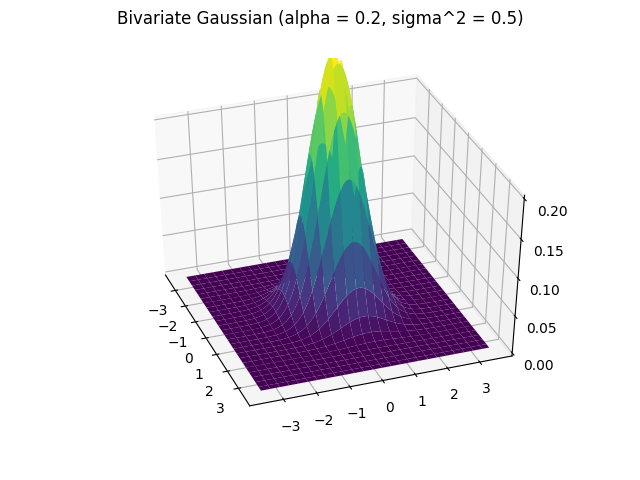
\includegraphics[width=\linewidth]{Bivariate Gaussian (alpha = 0.2, sigma^2 = 0.5).png}
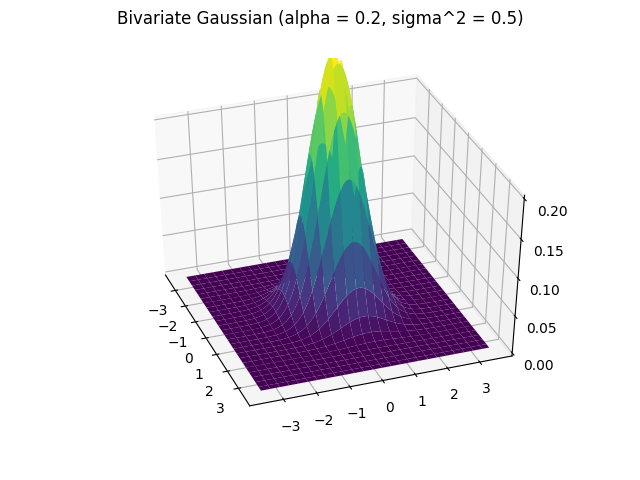
\includegraphics[width=\linewidth]{Bivariate Gaussian (alpha = 0.2, sigma^2 = 0.5).png}
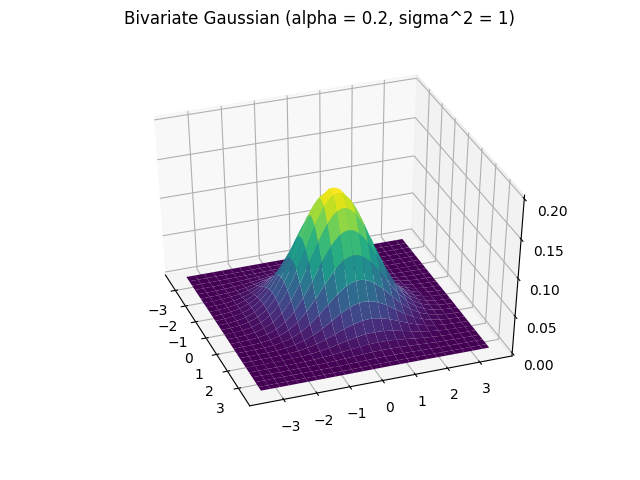
\includegraphics[width=\linewidth]{Bivariate Gaussian (alpha = 0.2, sigma^2 = 1).png}
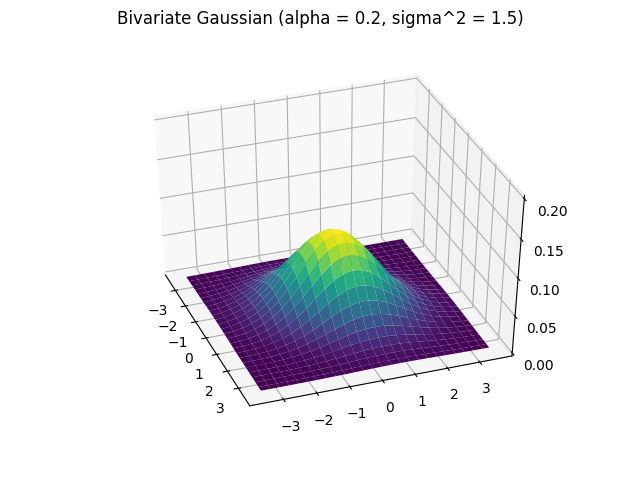
\includegraphics[width=\linewidth]{Bivariate Gaussian (alpha = 0.2, sigma^2 = 1.5).png}
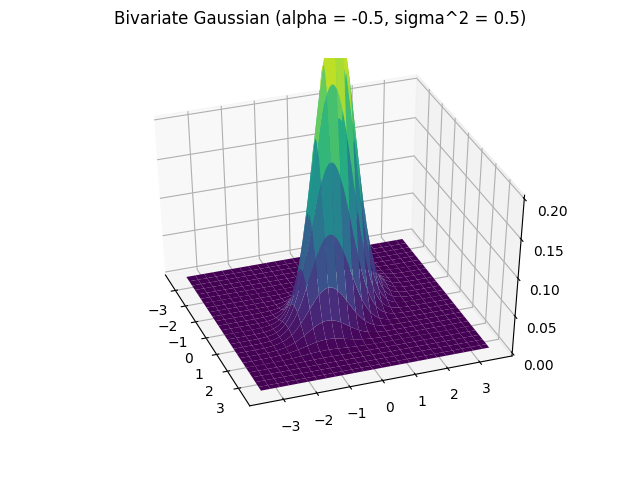
\includegraphics[width=\linewidth]{Bivariate Gaussian (alpha = -0.5, sigma^2 = 0.5).png}
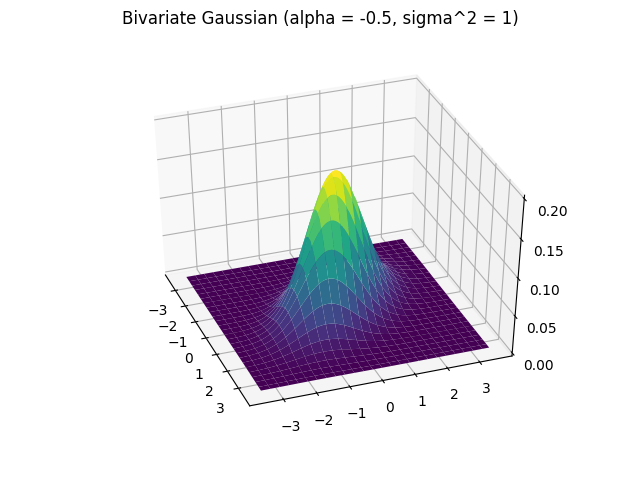
\includegraphics[width=\linewidth]{Bivariate Gaussian (alpha = -0.5, sigma^2 = 1).png}
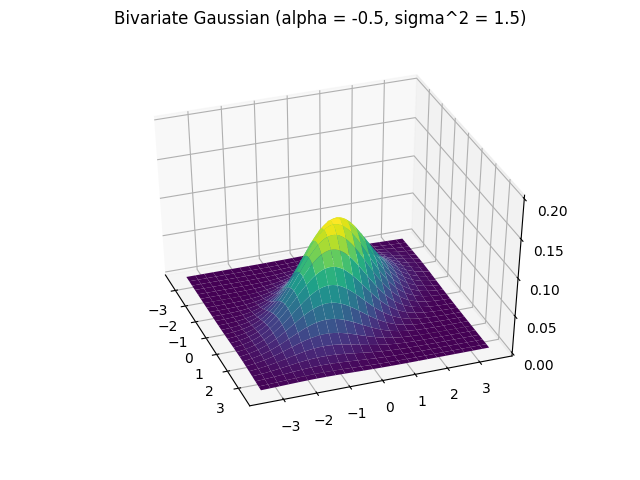
\includegraphics[width=\linewidth]{Bivariate Gaussian (alpha = -0.5, sigma^2 = 1.5).png}
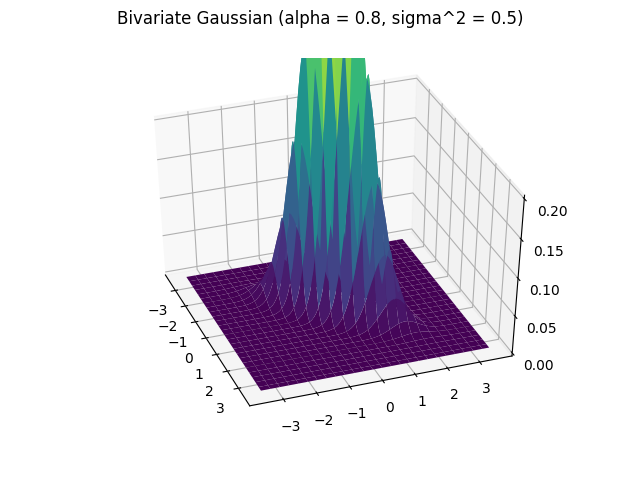
\includegraphics[width=\linewidth]{Bivariate Gaussian (alpha = 0.8, sigma^2 = 0.5).png}
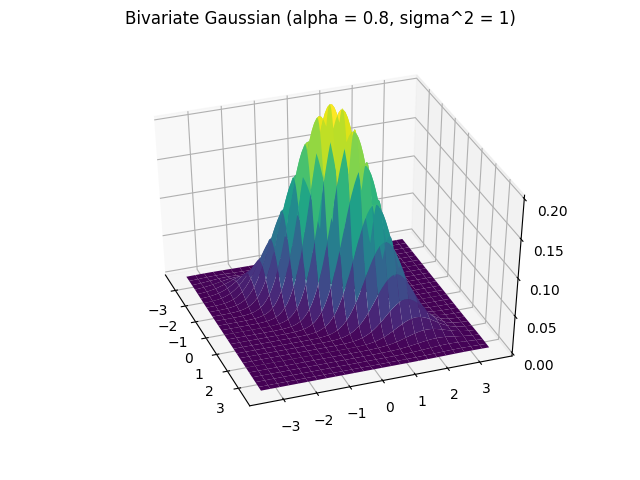
\includegraphics[width=\linewidth]{Bivariate Gaussian (alpha = 0.8, sigma^2 = 1).png}
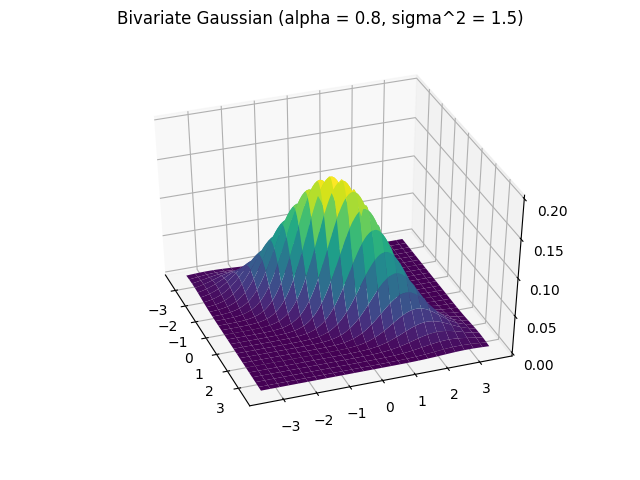
\includegraphics[width=\linewidth]{Bivariate Gaussian (alpha = 0.8, sigma^2 = 1.5).png}

\subsubsection{Bivariate Gaussian Marginals}
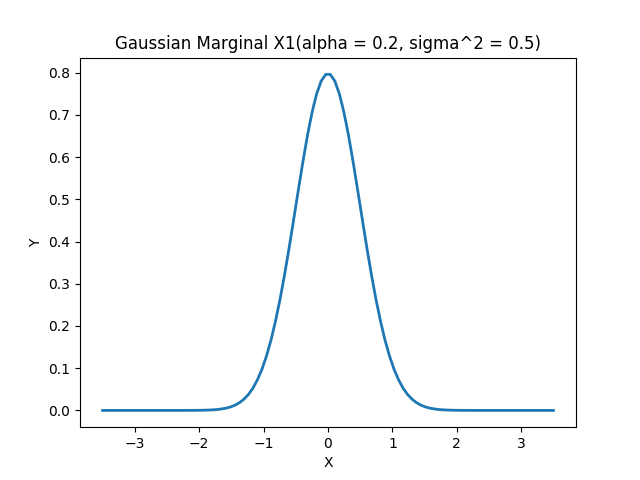
\includegraphics[width=\linewidth]{X1(alpha = 0.2, sigma^2 = 0.5).png}
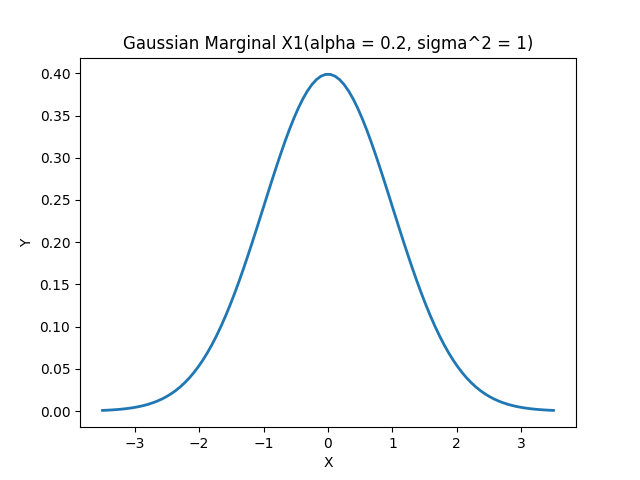
\includegraphics[width=\linewidth]{X1(alpha = 0.2, sigma^2 = 1).png}
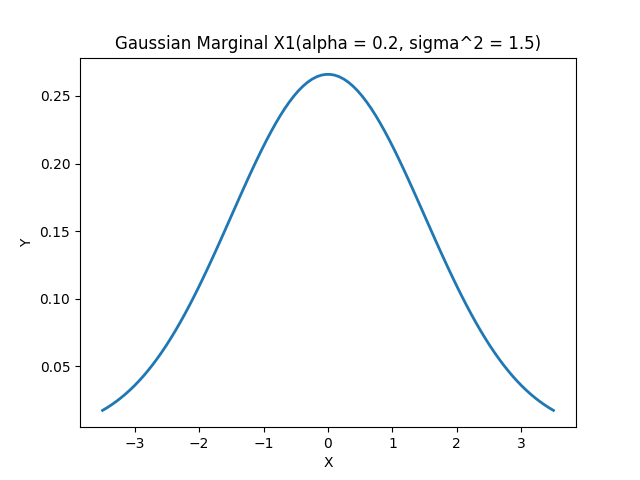
\includegraphics[width=\linewidth]{X1(alpha = 0.2, sigma^2 = 1.5).png}
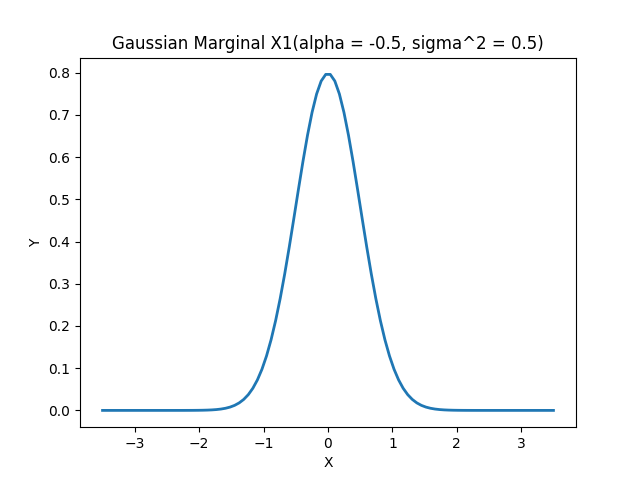
\includegraphics[width=\linewidth]{X1(alpha = -0.5, sigma^2 = 0.5).png}
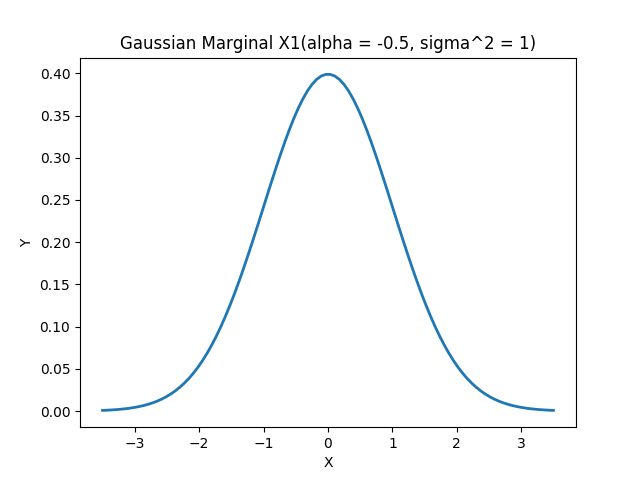
\includegraphics[width=\linewidth]{X1(alpha = -0.5, sigma^2 = 1).png}
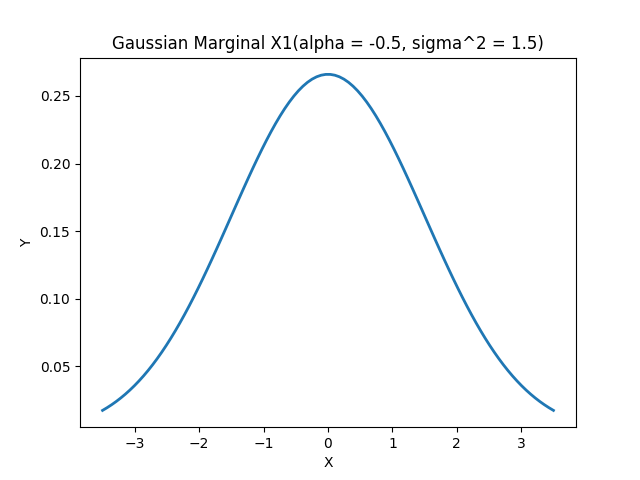
\includegraphics[width=\linewidth]{X1(alpha = -0.5, sigma^2 = 1.5).png}
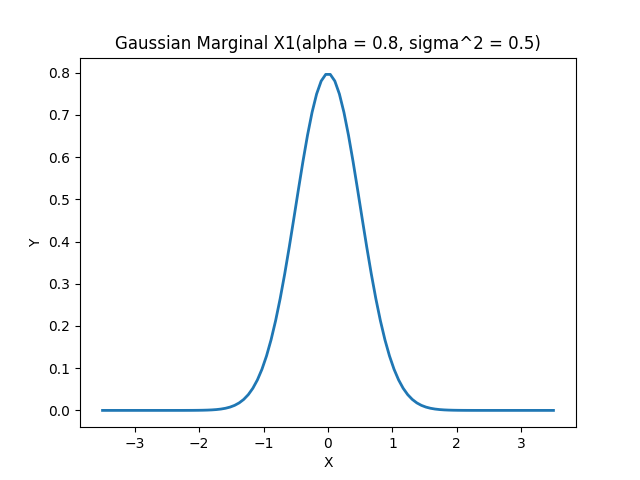
\includegraphics[width=\linewidth]{X1(alpha = 0.8, sigma^2 = 0.5).png}
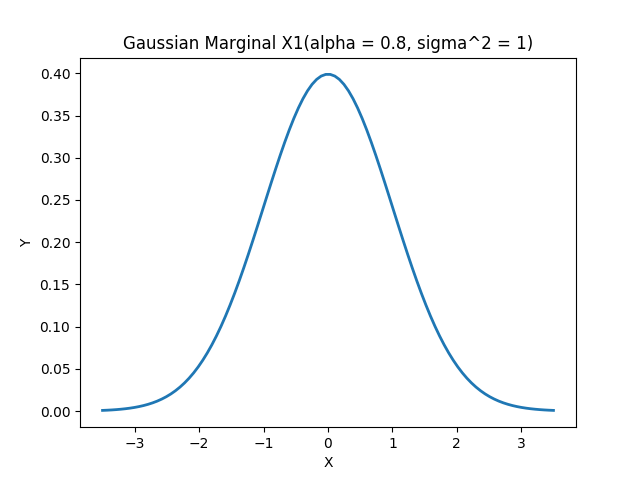
\includegraphics[width=\linewidth]{X1(alpha = 0.8, sigma^2 = 1).png}
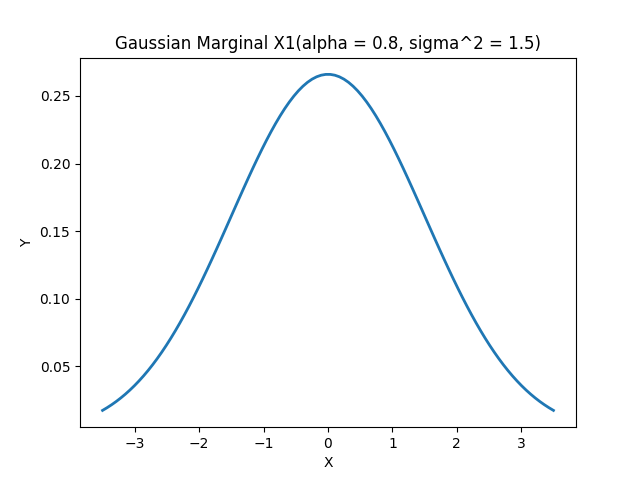
\includegraphics[width=\linewidth]{X1(alpha = 0.8, sigma^2 = 1.5).png}

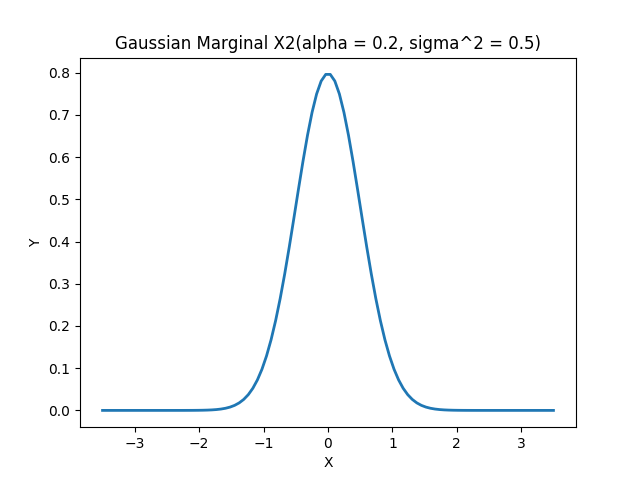
\includegraphics[width=\linewidth]{X2(alpha = 0.2, sigma^2 = 0.5).png}
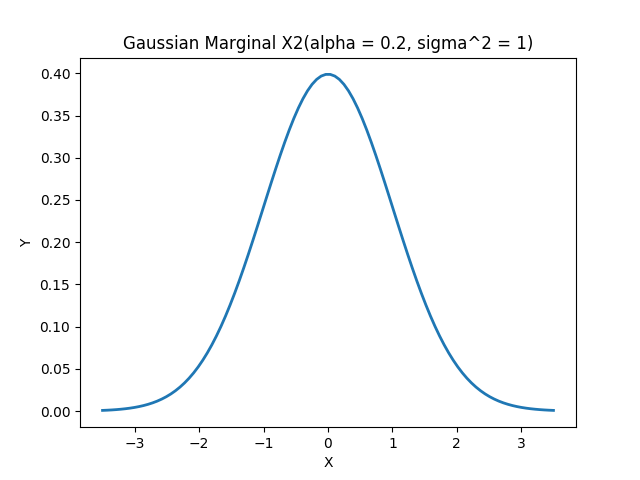
\includegraphics[width=\linewidth]{X2(alpha = 0.2, sigma^2 = 1).png}
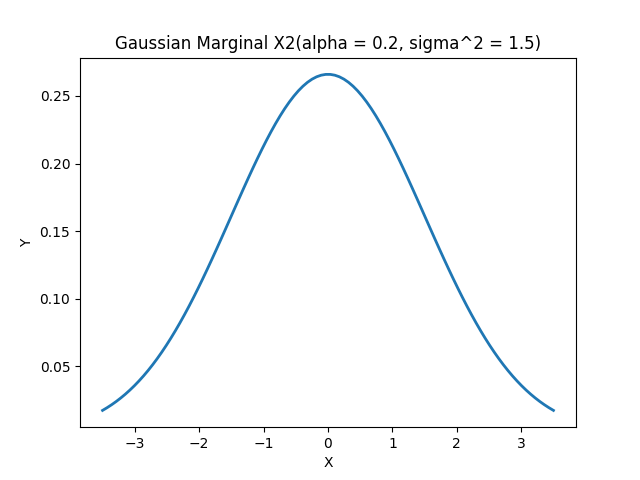
\includegraphics[width=\linewidth]{X2(alpha = 0.2, sigma^2 = 1.5).png}
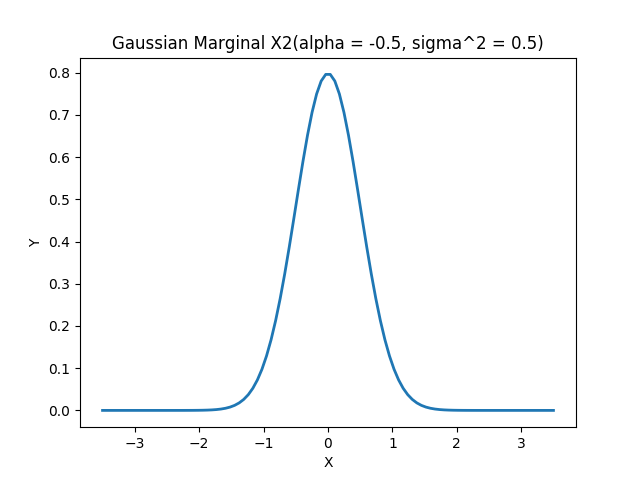
\includegraphics[width=\linewidth]{X2(alpha = -0.5, sigma^2 = 0.5).png}
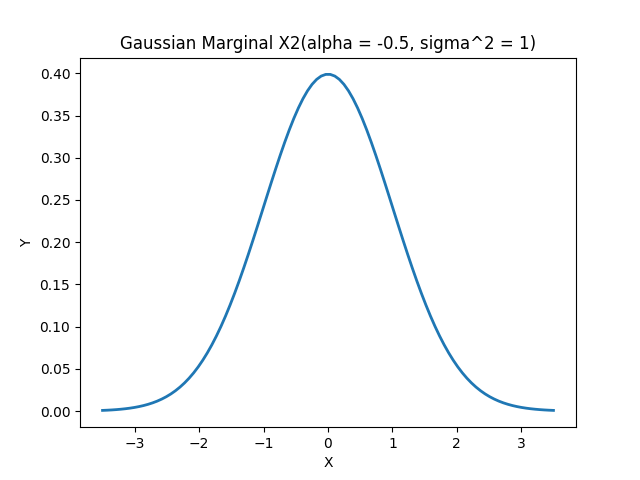
\includegraphics[width=\linewidth]{X2(alpha = -0.5, sigma^2 = 1).png}
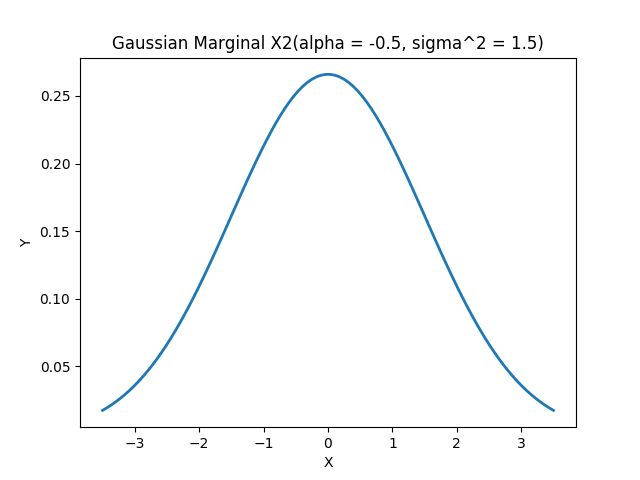
\includegraphics[width=\linewidth]{X2(alpha = -0.5, sigma^2 = 1.5).png}
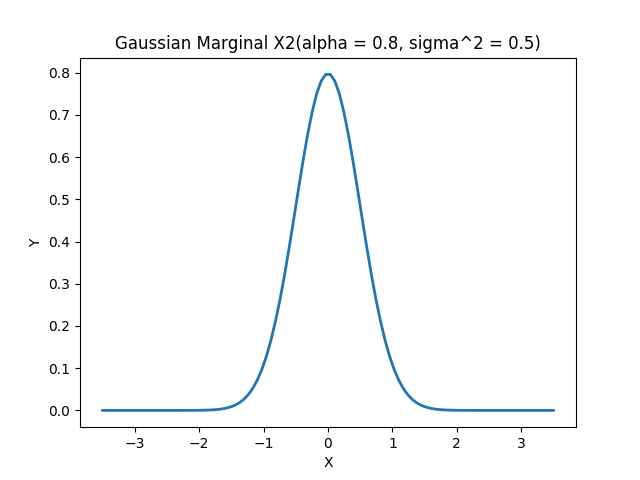
\includegraphics[width=\linewidth]{X2(alpha = 0.8, sigma^2 = 0.5).png}
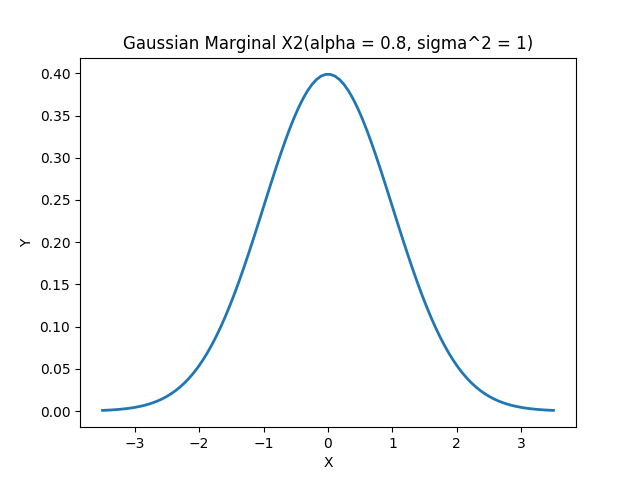
\includegraphics[width=\linewidth]{X2(alpha = 0.8, sigma^2 = 1).png}
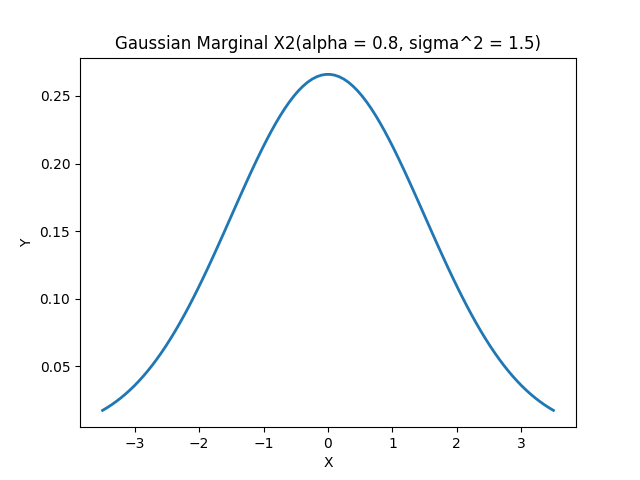
\includegraphics[width=\linewidth]{X2(alpha = 0.8, sigma^2 = 1.5).png}

\subsection{Task 3}
\subsubsection{Model Predictions}
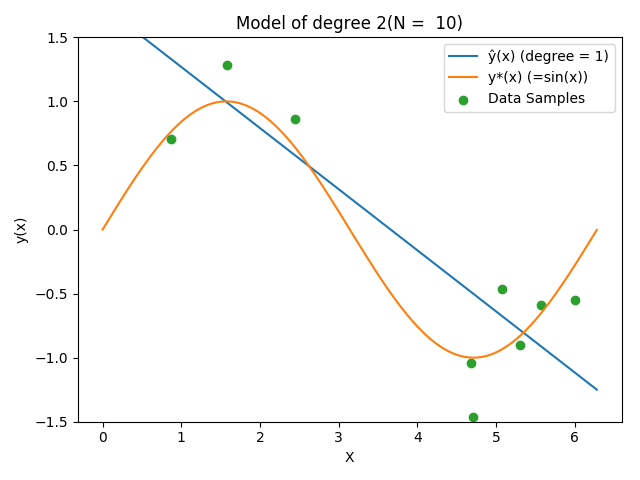
\includegraphics[width=\linewidth]{2.png}
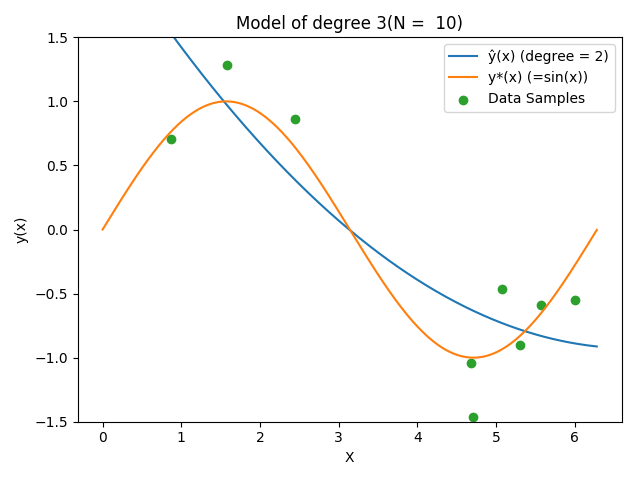
\includegraphics[width=\linewidth]{3.png}
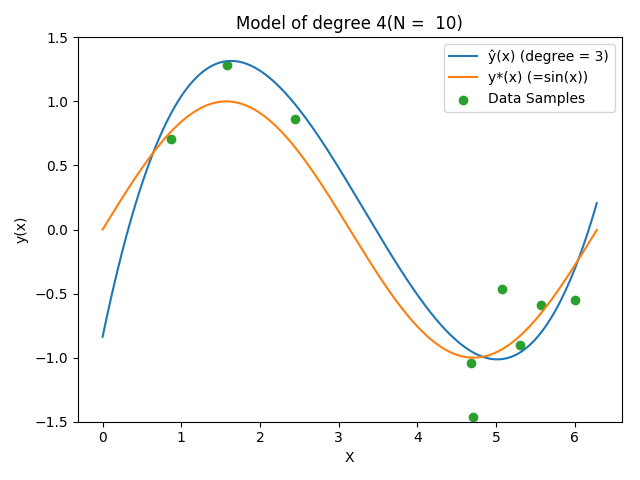
\includegraphics[width=\linewidth]{4.png}
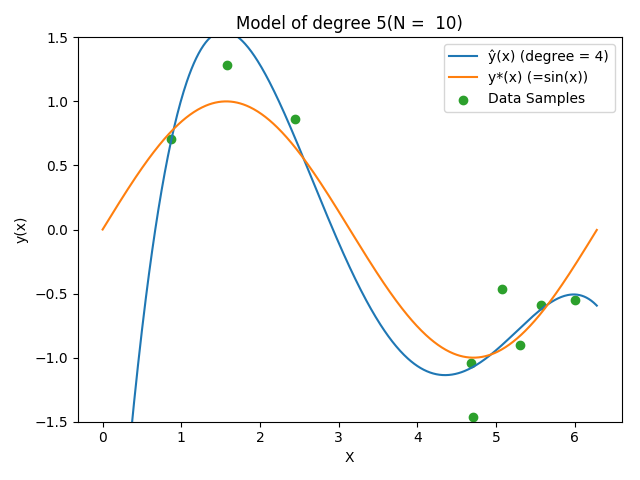
\includegraphics[width=\linewidth]{5.png}
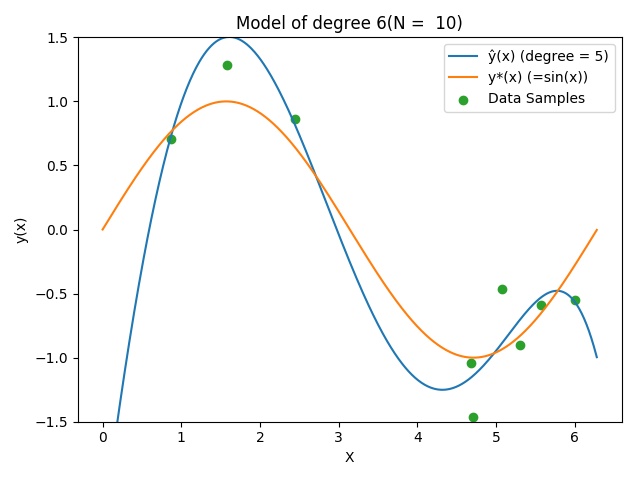
\includegraphics[width=\linewidth]{6.png}
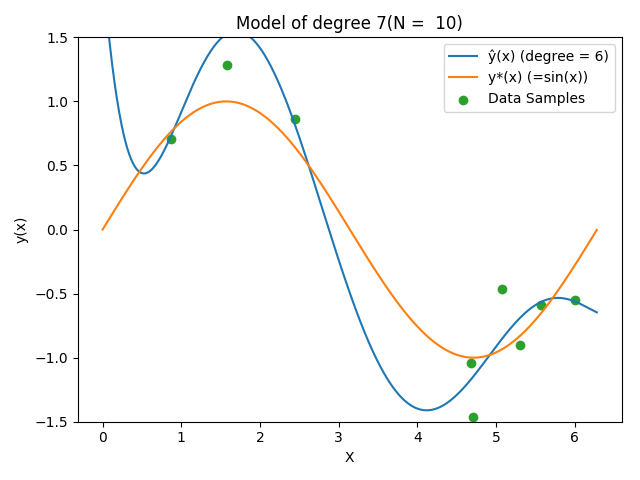
\includegraphics[width=\linewidth]{7.png}
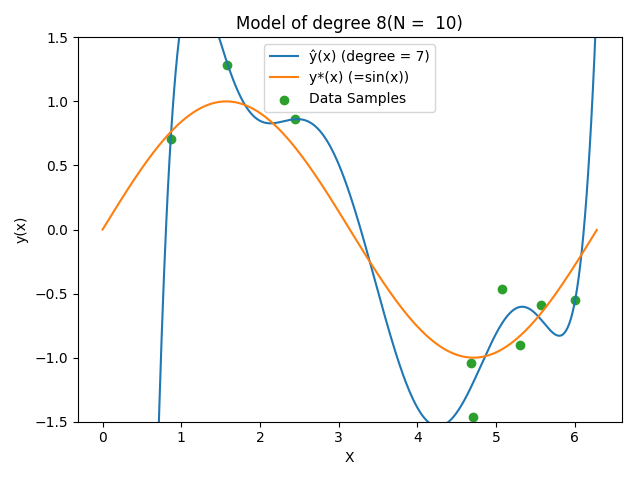
\includegraphics[width=\linewidth]{8.png}
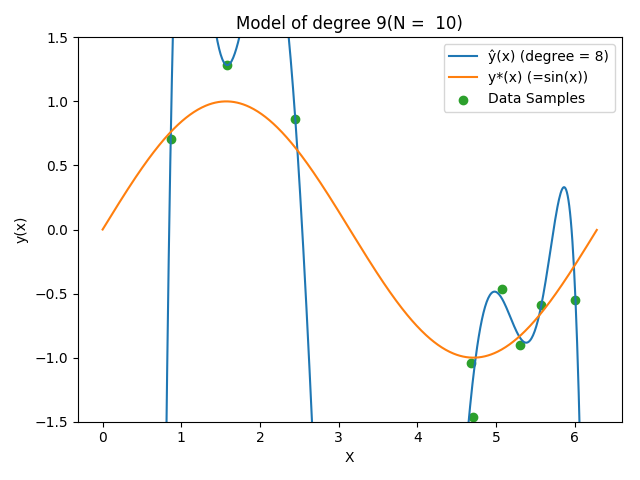
\includegraphics[width=\linewidth]{9.png}

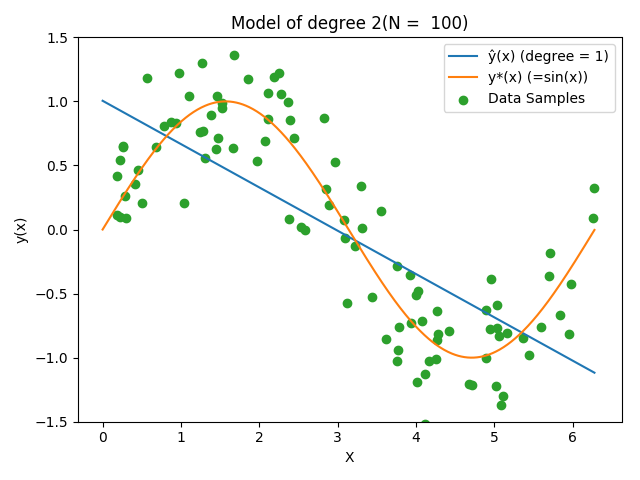
\includegraphics[width=\linewidth]{2_100.png}
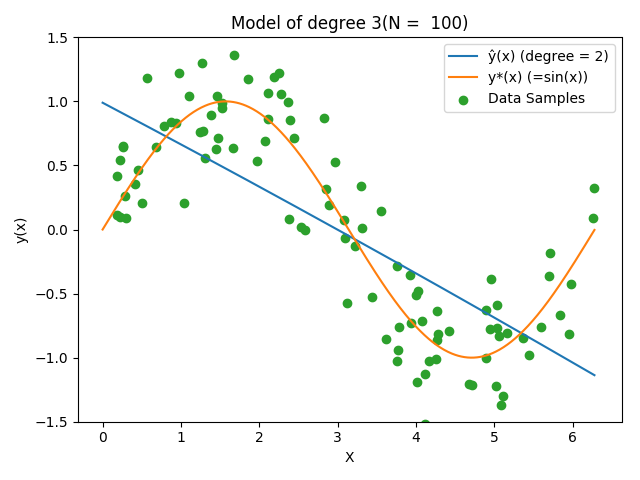
\includegraphics[width=\linewidth]{3_100.png}
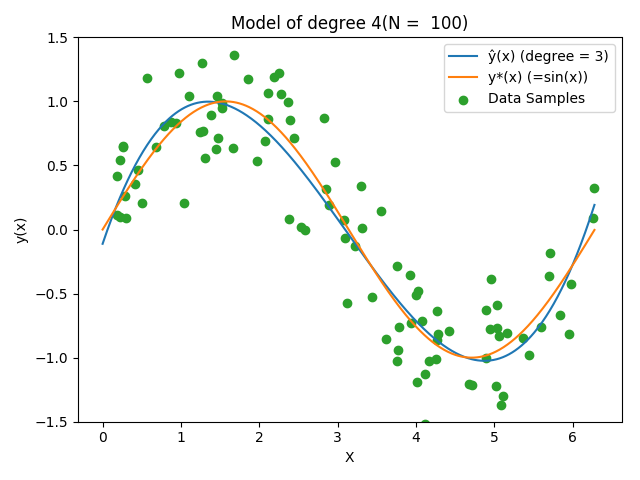
\includegraphics[width=\linewidth]{4_100.png}
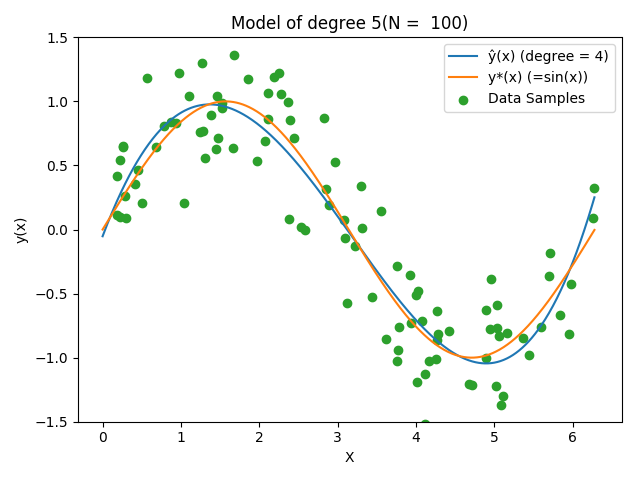
\includegraphics[width=\linewidth]{5_100.png}
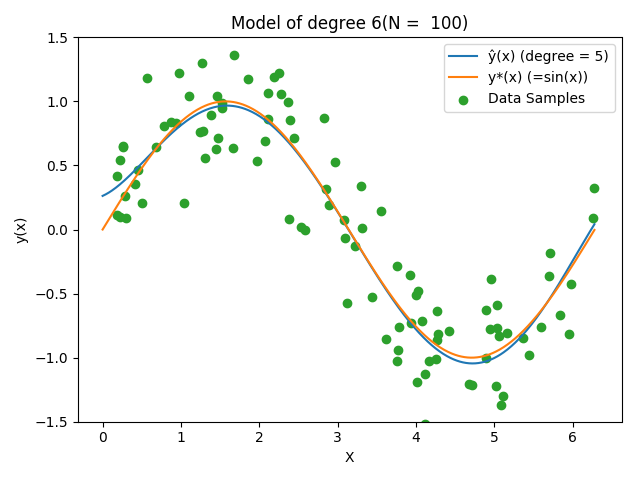
\includegraphics[width=\linewidth]{6_100.png}
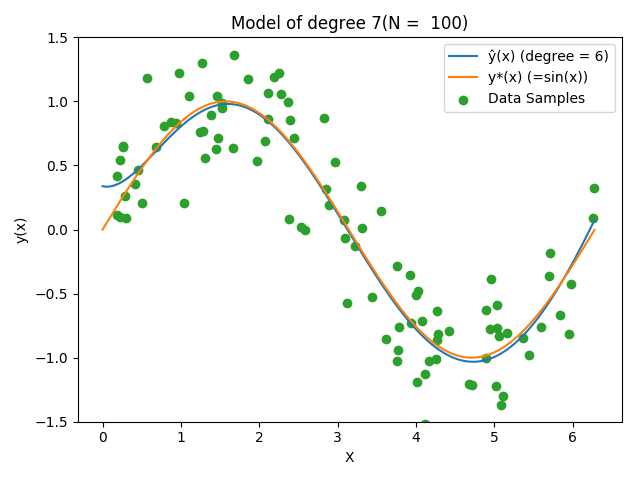
\includegraphics[width=\linewidth]{7_100.png}
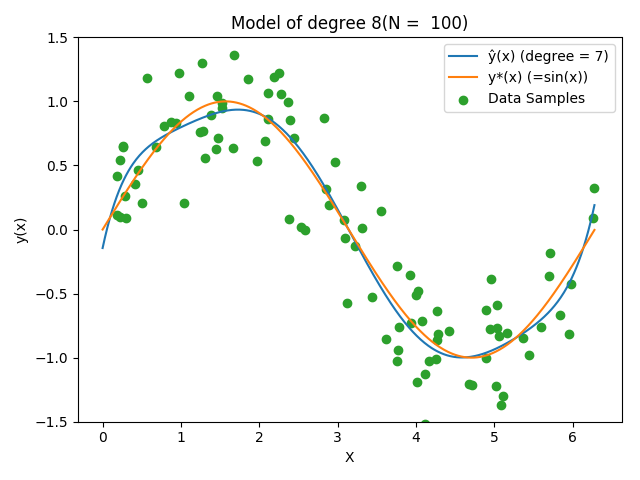
\includegraphics[width=\linewidth]{8_100.png}
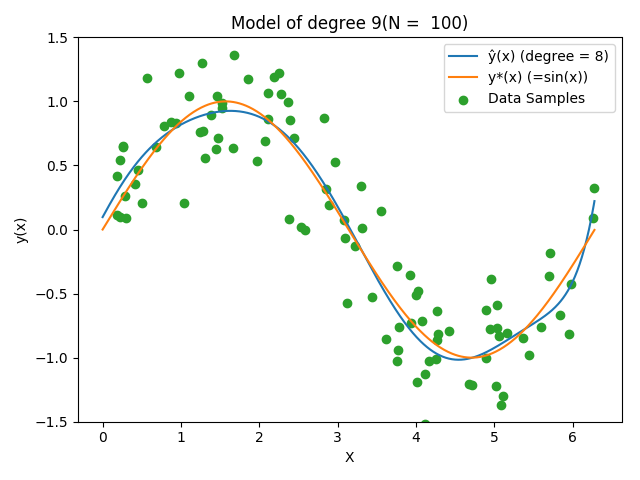
\includegraphics[width=\linewidth]{9_100.png}


\subsubsection{Risk}
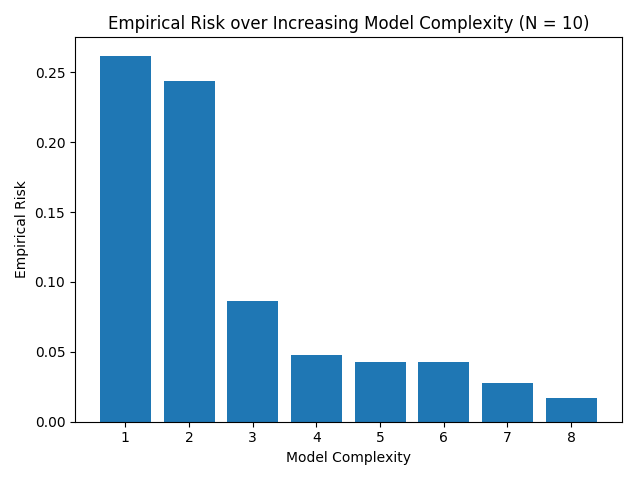
\includegraphics[width=\linewidth]{empirical.png}
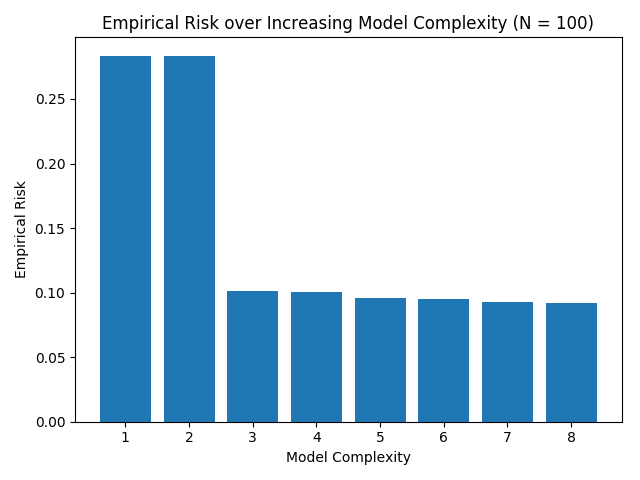
\includegraphics[width=\linewidth]{empirical_100.png}
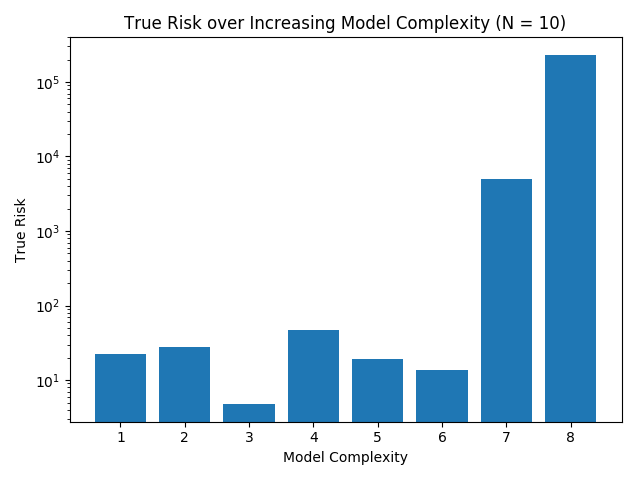
\includegraphics[width=\linewidth]{true.png}
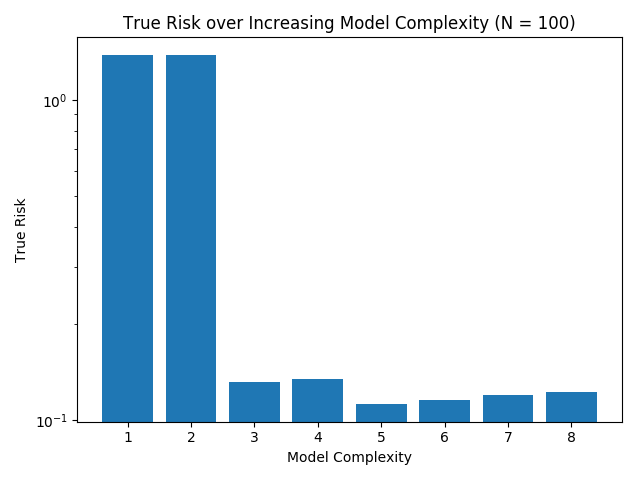
\includegraphics[width=\linewidth]{true_100.png}

\end{document}